\chapter{Vorauslegung}
\label{chap:Vorauslegung}

Zuerst wird eine analytische Vorauslegung basierend auf einer Abschätzung des Flugprofils durchgeführt.
Die Flugdaten kommen aus einer Trajektoriensimulation aus dem Simulationsprogramm OpenRocket, die vom Triebwerk-Subsystem durchgeführt wurde.
Diese Flugdaten in Abbildung \ref{fig:flugdaten_trajektoriensimulation} bilden eine Maximalabschätzung der aerodynamischen Aufheizung und Flugdauer durch
maximale Schub-Kraft und Dauer mit \SI{8}{\kilo\newton} für \SI{43}{\second}, die von \ac{blast} erreicht werden können.

\section{Anforderungen}

Da die Kühlung zeitgleich zu der Avionik entwickelt wurde, musste auf eine genaue Analyse aller Komponenten der Avionik verzichtet werden.
Stattdessen wurde anhand der bereits festgelegten Elektronik wie etwa dem Mikrocontroller STM32H743ZGT6, der auf den redundanten Flugcomputern verwendet wird,
die Auslegung durchgeführt.
Aus dem Datenblatt des Mikrocontrollers folgt eine maximale Sperrschichttemperatur von $T_\text{J} = \SI{125}{\degreeCelsius}$~\cite{STM32}
und ein Sperrschicht-Gehäuse-Wärmeleitwiderstand von $\Theta_\text{JC} = \SI{23,9}{\degreeCelsius\per\watt}$~\cite{STM32}. Mit einem konservativen
Sicherheitsfaktor von 1.5, um bisher unbekannte Bauteile zu berücksichtigen, folgt daraus $\Theta_\text{JC,safety} = \SI{35,85}{\degreeCelsius\per\watt}$
und eine maximale Gehäusetemperatur von $T_\text{C} = \SI{89,15}{\degreeCelsius}$. Im Kontext der Elektronik ist mit Gehäuse immer die
Oberseite der elektronischen Komponente gemeint.
Die Kühlung soll außerdem eine hohe Zuverlässigkeit haben, die durch Verwendung von ausschließlich passiven Bauteilen gewährleistet wird.
Dadurch kann aufwendiges und teures Testen und Verifizieren von aktiven Bauteilen mit mechanischer oder elektrischer Funktion vermieden werden, und es besteht bei
nicht nominalen Flügen eine geringere Ausfallwahrscheinlichkeit durch die inhärent größeren Toleranzen passiver Bauteile.

Dem Energieerhaltungssatz nach haben der \ac{fcc}, die Kameras und weitere Elektronik, die keine Leistung abgibt, gegenüber etwa
der \ac{pcdu} und Funkplatine, die Leistung in Form von Strom und elektromagnetischer Strahlung abgeben, einen Wirkungsgrad von
$\approx\SI{0}{\percent}$, da Logikoperationen physikalisch gesehen keine Arbeit sind. Resultierend wird der komplette Stromverbrauch
in Wärme umgewandelt.

\begin{table}
  \centering
  \caption{Leistung der Avionik}\label{tab:avionik_leistung}

  \begin{tabular}{lp{4cm}ll}
    \toprule[1pt]
    Komponente & Spannung \& Strom & Wirkungsgrad & Wärmestrom \\
    \midrule[0.5pt]

    STM32H743ZGT6 &
      \mbox{$V_\text{DD}=\SI{3,3}{\volt}$},\newline
      $I_\text{DD}=\SI{536}{\milli\ampere}$~\cite{STM32} &
      $\approx \SI{0}{\percent}$ & \SI{1,769}{\watt} \\
    $\dot{Q}_\text{ges}$ & & & \SI{7,075}{\watt}\\

    \midrule[0.5pt]
    RunCam Split 4 V2 &
      \mbox{$V_\text{DD}=\SI{5}{\volt}$},\newline
      $I_\text{DD}=\SI{450}{\milli\ampere}$~\cite{RunCam-Split4V2} &
      $\approx \SI{0}{\percent}$ & \SI{2,25}{\watt} \\
    $\dot{Q}_\text{ges}$ & & & \SI{9}{\watt}\\

    \midrule[0.5pt]
    Thebe-II &
      \mbox{$V_\text{DD}=\SI{3,6}{\volt}$},\newline
      $I_\text{DD}=\SI{500}{\milli\ampere}$~\cite{WE-ThebeII-UM-2024} &
      $\approx \SI{30}{\percent}$~\cite{WE-ThebeII-UM-2024} & \SI{1,3}{\watt} \\

    \midrule[0.5pt]
    \ac{pcdu} & & $\approx \SI{30}{\percent}$ & \SI{9,3}{\watt} \\

    \midrule[0.5pt]
    \midrule[0.5pt]
    $\dot{Q}_\text{ges, safety}$ & & & \SI{40}{\watt} \\

    \bottomrule[1pt]
  \end{tabular}
\end{table}

Die Leistung der Avionik in Tabelle~\ref{tab:avionik_leistung} ergibt sich durch den Maximalverbrauch der \ac{fcc}-Mikrocontroller
(STM32H743ZGT6) bei maximaler Taktfrequenz (\SI{400}{\mega\hertz}) und vollständig aktiver Peripherie, der Kameras und einer
Abschätzung der restlichen Komponenten, für die keine exakten Werte vorhanden sind. Der aus Tabelle~\ref{tab:avionik_leistung} resultierende gesamte Wärmestrom
der Avionik mit \SI{40}{\watt} ist mit einem gewöhnlichen Laptop vergleichbar.

\begin{figure}
    \centering

    % Column 1, Row 1
    \begin{subfigure}{0.48\textwidth}
        \centering
        \includegraphics[width=\linewidth]{../../Code/acceleration_over_time.pdf}
        \caption{Beschleunigung während Flug}
        \label{fig:acceleration_over_time}
    \end{subfigure}
    \hfill
    % Column 2, Row 1
    \begin{subfigure}{0.48\textwidth}
        \centering
        \includegraphics[width=\linewidth]{../../Code/altitude_over_time.pdf}
        \caption{Flughöhe}
        \label{fig:altitude_over_time}
    \end{subfigure}

    \vspace{1em}

    % Column 1, Row 2
    \begin{subfigure}{0.48\textwidth}
        \centering
        \includegraphics[width=\linewidth]{../../Code/pressure_over_time.pdf}
        \caption{Statischer Luftdruck während Flug}
        \label{fig:pressure_over_time}
    \end{subfigure}
    \hfill
    % Column 2, Row 2
    \begin{subfigure}{0.48\textwidth}
        \centering
        \includegraphics[width=\linewidth]{../../Code/temperature_over_time.pdf}
        \caption{Statische Lufttemperatur während Flug}
        \label{fig:temperature_over_time}
    \end{subfigure}

    \vspace{1em}

    % Column 1, Row 3
    \begin{subfigure}{0.48\textwidth}
        \centering
        \includegraphics[width=\linewidth]{../../Code/velocity_over_time.pdf}
        \caption{Geschwindigkeit während Flug}
        \label{fig:velocity_over_time}
    \end{subfigure}
    \hfill
    % Column 2, Row 3
    \begin{subfigure}{0.48\textwidth}
        \centering
        \includegraphics[width=\linewidth]{../../Code/dynp_during_flight.pdf}
        \caption{Dynamischer Druck während Flug}
        \label{fig:dynp_over_time}
    \end{subfigure}

    \caption{Flugdaten der Trajektoriensimulation.}\label{fig:flugdaten_trajektoriensimulation}
\end{figure}

\section{Thermale Schnittstelle}\label{sec:thermale_schnittstelle}

Um mit der Abwärme der Avionik umgehen zu können, muss sie effektiv gesammelt und abtransportiert werden.
Oft werden in der Luft- und Raumfahrtindustrie Kühlkreisläufe mit einem Arbeitsfluid verwendet, etwa bei der internationalen Raumstation ISS~\cite{ISS-ATCS}.
Diese benötigen jedoch meist bewegliche Bauteile wie Pumpen, welche die Ausfallwahrscheinlichkeit erhöhen. Alternativ gibt es auch
Möglichkeiten, durch erzwungene Konvektion ein Arbeitsfluid anzutreiben oder Materialien mit hoher Wärmeleitfähigkeit
zu verwenden. Beide Methoden bieten in Kombination eine leichte Integrierbarkeit und geringen Wärmeleitwiderstand,
ohne bewegliche Teile zu verwenden.

Das thermale Interface wird auf Systemebene analysiert, da eine Entwicklung auf Ebene des \ac{pcb} wie bereits erläutert nicht
möglich ist, ohne die vollständig entwickelte Elektronik.

\subsection{Heatpipes}\label{sec:waermerohre}

Heatpipes (Wärmerohre) sind eine Möglichkeit, durch erzwungene Konvektion Wärme zu transportieren. Reguläre Heatpipes
sind vollständig geschlossene Rohre mit einer Flüssigkeit im Inneren und einer Kapillarstruktur an der Innenwand,
so dass ein freier Kanal in der Mitte bleibt. Bei der Wärmequelle
verdampft die Flüssigkeit aus der Kapillarstruktur und bei der Wärmesenke kondensiert sie wieder, wodurch der resultierende Massenstrom einen
Kreislauf bildet. Besonders effektiv sind Heatpipes durch die Nutzung der Verdampfungsenthalpie beim Flüssig-Gas-Übergang an der Wärmequelle,
wodurch sehr hohe Wärmestromdichten erreicht werden können. Eine schematische Darstellung einer Heatpipe zeigt Abbildung~\ref{fig:waermerohr}.

Eine Weiterentwicklung davon sind Loop Heatpipes, die, wie der Namen bereits impliziert, einen Kreislauf bilden, indem es eine
separate Flüssig- und Dampfleitung gibt, die jeweils am Verdampfer und Kondensator miteinander verbunden sind.
Besonders von Vorteil sind Loop Heatpipes, wenn größere Distanzen überbrückt werden müssen, oder eine relativ zuverlässige
Funktion unabhängig von Orientierung und Gravitation gebraucht wird. Aufgrund der erhöhten Komplexität von Loop Heatpipes, der Möglichkeit,
die Orientierung der Heatpipes frei zu bestimmen, den relativ geringen Distanzen innerhalb der Avioniksektion und dem Mangel an kommerziell erhältlichen
Loop Heatpipes wird eine reguläre Heatpipe gewählt.


\begin{figure}
  \centering
  \begin{tikzpicture}
    \draw[thick] (-5,0) arc [start angle=90, end angle=270, x radius=1.5cm, y radius= 1.5cm]; % Kappen
    \draw[thick] (5,0) arc [start angle=90, end angle=-90, x radius=1.5cm, y radius= 1.5cm];

    \draw[thick] (-5,0) -- (5,0); % hülle
    \draw[thick] (-5,-3) -- (5,-3);

    \draw[dashed] (-5,0) rectangle (5,-1); % Wick Abgrenzung
    \draw[dashed] (-5,-2) rectangle (5,-3);

    \draw[->, thick, -{Stealth[length=0.25cm]}] (-1,-1.75) -- node [midway, above] {Dampfstrom} (1,-1.75); % Dampf Pfeil
    \draw[->, thick, -{Stealth[length=0.25cm]}] (1,-2.75) -- node [midway, above] {Flüssigstrom}(-1,-2.75); % Flüssigkeitspfeil
    \draw[->, thick, -{Stealth[length=0.25cm]}] (1,-0.5) -- (-1,-0.5); % Flüssigkeitspfeil

    \node at (-4,-4) [style={single arrow, draw}, minimum height=0.5cm, minimum width=1.5cm, shape border rotate=90, thick]{$\dot{Q}$}; % Wärmestrom pfeil
    \node at (4,-3.75) [style={single arrow, draw}, minimum height=0.5cm, minimum width=1.5cm, shape border rotate=270, thick]{$\dot{Q}$}; % Wärmestrom pfeil
    
    \draw[->, thick, -{Stealth[length=0.25cm]}] (-4,0.25) node [above=1pt] {Kapillarstruktur} -- (-3,-0.5); % Kapillar Pfeil
    \draw[->, thick, -{Stealth[length=0.25cm]}] (-4,0.25) -- (-3,-2.5);
  \end{tikzpicture}
  \caption{Heatpipe Aufbau und Funktionsweise.}\label{fig:waermerohr}
\end{figure}

Ein wichtiger Aspekt von Heatpipes ist, dass der Wärmeleitwiderstand durch Biegungen und Anbindung von mehreren Quellen um bis zu \SI{100}{\percent}
steigen kann \cite{Mooney-2020}. Auch wenn Heatpipes konvektiv arbeiten, ist bei deren Wärmeübertragung vom Wärmeleitwiderstand die Rede.
Des Weiteren hängt besonders bei regulären Heatpipes der Wärmeleitwiderstand von der effektiven Beschleunigung ab,
da die höhere Dichte der Flüssigphase eine beschleunigende Wirkung auf die Konvektion hat, wenn die Wärmequelle unten orientiert ist. Sollte die Heatpipe jedoch
\glqq über Kopf \grqq{} arbeiten, sodass die Wärmequelle oben orientiert ist, muss die Konvektion gegen die Beschleunigung arbeiten und verliert Leistung bzw. hat
einen erhöhten Wärmeleitwiderstand.

Ausgewählt wurde die QG-SHP-D5-400MN Heatpipe von Quick-Ohm Küpper \& Co. GmbH aus Kupfer mit Mesh-Gewebe als Kapillarstruktur von \SI{400}{\milli\meter} Länge und
\SI{5}{\milli\meter} Durchmesser. Diese Heatpipe kann eine Leistung von \SI{40}{\watt} übertragen.

Weiterhin wird die Heatpipe als \ac{rom} mit einem einfachen Widerstand ersetzt, der dem Wärmeleitwiderstand von $R_\mathrm{Heatpipe} = \SI{0,3}{\kelvin\per\watt}$ aus dem Datenblatt~\cite{QuickOhm-Heatpipe-5x400} entspricht.
Dadurch wird eine sehr komplexe Modellierung abhängig von Temperaturen, Biegungen, Ausrichtung, Beschleunigung und Anzahl an Wärmequellen sowie deren Leistung und Positionen vermieden.

\subsection{Wärmeleitbänder}\label{sec:waermebaender}

Um die Elektronik mit der Heatpipe zu verbinden, werden Wärmeleitbänder aus verschiedenen Materialien analysiert.
Wärmeleitbänder sind flexible Verbindungsteile mit hoher Wärmeleitfähigkeit, die Wärmebrücken zwischen mehreren Bauteilen gewährleisten.
\ac{pgs} ist gegenüber herkömmlichen Materialien besonders interessant durch die extrem hohe Wärmeleitfähigkeit innerhalb der Ebene,
da diese der Ebene der Molekülstruktur des Graphit entspricht. Außerdem ist es ein relativ flexibles Material bei einer üblichen Dicke von $\approx \SIrange{10}{100}{\micro\meter}$.
Ein Nachteil von \ac{pgs} ist die im Kontrast zur Ebene sehr niedrige Wärmeleitfähigkeit durch die Ebene infolge von wenigen
molekularen Brücken zwischen den Gitterstrukturen. Dementsprechend werden \ac{pgs} und andere Arten von Graphit-Folien hauptsächlich zur
Wärmeverteilung auf der Oberfläche von Bauteilen verwendet, um Wärmestromdichten zu verringern und homogenere Temperaturverteilungen zu erreichen.

Das effektive Erhöhen des Querschnitts von \ac{pgs} durch Schichtung mehrerer Folien aufeinander ermöglicht es jedoch, die hohe
Wärmeleitfähigkeit in der Ebene auch zum thermischen Koppeln mehrerer Bauteile zu verwenden. Diese Anwendung hat besonders in der 
Raumfahrt durch ermöglichte Masseneinsparungen großes Potential. Eine kommerzielle Reihe solcher Wärmeleitbänder aus gängigen Materialien zeigt Abbildung~\ref{fig:thermalstraps_commercial}.
Der Tabelle~\ref{tab:strap_materials} nach ist \ac{pgs} der beste Kompromiss für die geforderten Eigenschaften. Um jedoch zu vermeiden, dass
bei starken Vibrationen aufgrund der Flexibilität des \ac{pgs} Kontakt mit der Elektronik und mögliche Kurzschlüsse entstehen, muss das Wärmeleitband mit einer elektrisch
isolierenden Ummantelung versehen werden.

\begin{figure}
  \centering
  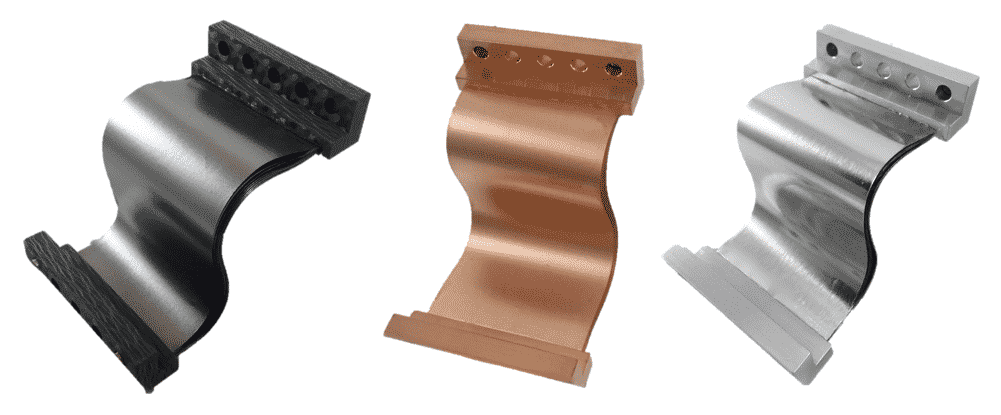
\includegraphics[width=\textwidth]{thermal_straps_commercial.png}
  \caption{Kommerziell erhältliche Wärmeleitbänder aus \acs{pgs} (links), Kupfer und Aluminium~\cite{Thermal-Straps}.}\label{fig:thermalstraps_commercial}
\end{figure}

\definecolor{good}{RGB}{200,255,200}   % hellgrün
\definecolor{medium}{RGB}{255,255,200} % hellgelb
\definecolor{bad}{RGB}{255,200,200}    % hellrot

\begin{table}
  \centering
  \caption{Ampelbewertung von Materialien für Wärmeleitbänder.}\label{tab:strap_materials}

  % 1. Spalte als Box-Spalte, damit \\ innerhalb der ZELLE umbricht
  \begin{tabular}{>{\raggedright\arraybackslash}m{3cm} m{3.2cm} m{3.2cm} m{3cm}}
    \toprule[1pt]
    Eigenschaft & Kupfer\cite{Thermtest-DB} & Aluminium\cite{Thermtest-DB} & \acs{pgs} \nobreak{(Graphit)}\cite{HPMS-PGS} \\
    \midrule[0.5pt]

    \makecell[l]{Wärmeleit-\\fähigkeit\\in Ebene}
      & \cellcolor{medium}\SI{397,48}{\watt\per\meter\per\kelvin}
      & \cellcolor{bad}\SI{225,94}{\watt\per\meter\per\kelvin}
      & \cellcolor{good}\SIrange{1050}{1800}{\watt\per\meter\per\kelvin} \\

    \makecell[l]{Wärmeleit-\\fähigkeit\\durch Ebene}
      & \cellcolor{good}\SI{397,48}{\watt\per\meter\per\kelvin}
      & \cellcolor{medium}\SI{225,94}{\watt\per\meter\per\kelvin}
      & \cellcolor{bad}\SIrange{10}{26}{\watt\per\meter\per\kelvin} \\

    Dichte
      & \cellcolor{bad}\SI{8940}{\kilogram\per\cubic\meter}
      & \cellcolor{medium}\SI{2698}{\kilogram\per\cubic\meter}
      & \cellcolor{good}\SIrange{1500}{2100}{\kilogram\per\cubic\meter} \\

    \makecell[l]{Elektrische\\Isolation}
      & \cellcolor{bad}Schlecht
      & \cellcolor{bad}Schlecht
      & \cellcolor{bad}Schlecht \\
    \bottomrule[1pt]
  \end{tabular}
\end{table}

Aufgrund der höchsten Wärmeleitfähigkeit in der Ebene des \ac{pgs} HGS-012 der Firma HPMS Graphite~\cite{HPMS-PGS} wurde dieses ausgewählt.
Um ein verwendbares Wärmeleitband zu konstruieren, soll dieses aus 32 Schichten bestehen, \SI{4}{\centi\meter} breit und 
\SI{10}{\centi\meter} lang sein, wodurch es ermöglicht werden soll, dass die Heatpipe möglichst Biegungsfrei verlaufen kann.
Die Anbindungen bzw. Endstücke der Wärmeleitbänder sowie Kontaktwiederstände durch Klebstoffe oder ähnliche Verbindungsmethoden werden ignoriert.
Der Wärmeleitwiderstand ergibt sich durch Einsetzen von Gleichung \ref{eq:fourier_1d} in \ref{eq:waermewiederstand}:

\begin{equation*}
  R_\mathrm{Wärmeleitband} = \frac{\Delta x}{\lambda A}
\end{equation*}

Mit $\Delta x = \SI{10}{\centi\meter}$, $\lambda = \SI{1800}{\watt\per\meter\kelvin}$ und $A = 32 \cdot \SI{0,012}{\milli\meter} \cdot \SI{4}{\centi\meter} = \SI{15,36}{\milli\meter\squared}$
ergibt sich $R_\mathrm{Wärmeleitband} = \SI{3,617}{\kelvin\per\watt}$.

\subsection{Gesamte Schnittstelle}\label{sec:gesamte_schnittstelle}

Mittels einer Kombination von \ac{pgs} und Heatpipe kann eine Wärmebrücke gebildet werden, die den Wärmeleitwiderstand
minimiert. Eine schematische Darstellung der thermalen Schnittstelle ist in Abbildung~\ref{fig:thermale_schnittstelle} zu sehen.

Wenn angenommen wird, dass die Avionik aus vier separaten \ac{pcb} mit einer Gesamtleistung von \SI{40}{\watt}~(\ref{tab:avionik_leistung}) besteht, müssen pro Wärmeleitband \SI{10}{\watt} übertragen werden.
Dabei entsteht nach Gleichung~\ref{eq:waermewiederstand} eine Temperaturerhöhung über das Wärmeleitband von $\Delta T_\mathrm{Wärmeleitband} = \SI{10}{\watt} \cdot \SI{3,617}{\watt\per\kelvin} = \SI{36,17}{\kelvin}$.
Die Heatpipe überträgt den vollständigen Wärmestrom und hat eine Temperaturerhöhung von $\Delta T_\mathrm{Heatpipe} = \SI{40}{\watt} \cdot \SI{0,3}{\watt\per\kelvin} = \SI{12}{\kelvin}$.

Von der Quelle bis zur Senke ergibt sich also ein Temperaturgradient von $\Delta T_\mathrm{ges} = \Delta T_\mathrm{Heatpipe} + \Delta T_\mathrm{Wärmeleitband} = \SI{48,17}{\kelvin}$.
Eine schematische Darstellung der Schnittstelle sieht man in Abbildung~\ref{fig:thermale_schnittstelle}. Für die nötige Temperatur an der Senke
erhält man $T_\mathrm{Senke} = T_C - \Delta T_\mathrm{ges} = \SI{314,13}{\kelvin}$. Die Masse der Schnittstelle wird nicht berücksichtigt, da diese
unabhängig von der Kühlung der Senke notwendig ist und stark von der Elektronik bzw. deren Platzierung abhängt.

\begin{figure}
  \centering
  \begin{tikzpicture}
    \node at (0,0) [style={single arrow, draw}, minimum height=0.5cm, minimum width=1.5cm, shape border rotate=90, thick]{$\dot{Q}$}; % Wärmestrom pfeil

    \draw[thick] (0,-1) -- (0,-3.1);

    \draw[thick] (0,-3.1) -- (-0.2,-3.2); % heatpipe resistor
    \draw[thick] (-0.2,-3.2) -- (0.2,-3.4);
    \draw[thick] (0.2,-3.4) -- (-0.2,-3.6);
    \draw[thick] (-0.2,-3.6) -- (0.2,-3.8);
    \draw[thick] (0.2,-3.8) -- (-0.2,-4);
    \draw[thick] (-0.2,-4) -- (0.2,-4.2);
    \draw[thick] (0.2,-4.2) -- (0,-4.3);

    \node[rotate=90] at (-0.5,-3.7) {Heatpipe};
    \node at (2.5,-3.7) {$R_{\mathrm{Heatpipe}} = \SI{0,3}{\kelvin\per\watt}$};

    \draw[thick] (0,-4.3) -- (0,-6.4);

    \draw[thick] (0,-6.4) -- (2.1,-6.4);

    \fill (0,-6.4) circle (1.5pt); %knotenpunkt

    \begin{scope}[shift={(-1,-6.4)}, rotate=90]
      \draw[thick] (0,-3.1) -- (-0.2,-3.2); % thermal strap resistor
      \draw[thick] (-0.2,-3.2) -- (0.2,-3.4);
      \draw[thick] (0.2,-3.4) -- (-0.2,-3.6);
      \draw[thick] (-0.2,-3.6) -- (0.2,-3.8);
      \draw[thick] (0.2,-3.8) -- (-0.2,-4);
      \draw[thick] (-0.2,-4) -- (0.2,-4.2);
      \draw[thick] (0.2,-4.2) -- (0,-4.3);
    \end{scope}


    \node at (2.7,-5.9) {Wärmeleitband};
    \node at (2.7,-6.9) {$R_{\mathrm{Wärmeleitband}} = \SI{3,617}{\kelvin\per\watt}$};

    \draw[thick] (3.3,-6.4) -- (5.4,-6.4);

    \node at (6.4,-6.4) [style={single arrow, draw}, minimum height=0.5cm, minimum width=1.5cm, shape border rotate=180, thick]{$\frac{\dot{Q}}{4}$}; % Wärmestrom pfeil

    \draw[thick] (0,-6.4) -- (0,-8.4);

    \draw[thick] (0,-8.4) -- (2.1,-8.4);

    \fill (0,-8.4) circle (1.5pt);% knotenpunkt 2

    \begin{scope}[shift={(-1,-8.4)}, rotate=90]
      \draw[thick] (0,-3.1) -- (-0.2,-3.2); % thermal strap resistor 2
      \draw[thick] (-0.2,-3.2) -- (0.2,-3.4);
      \draw[thick] (0.2,-3.4) -- (-0.2,-3.6);
      \draw[thick] (-0.2,-3.6) -- (0.2,-3.8);
      \draw[thick] (0.2,-3.8) -- (-0.2,-4);
      \draw[thick] (-0.2,-4) -- (0.2,-4.2);
      \draw[thick] (0.2,-4.2) -- (0,-4.3);
    \end{scope}

    \node at (2.7,-7.9) {Wärmeleitband};
    \node at (2.7,-8.9) {$R_{\mathrm{Wärmeleitband}} = \SI{3,617}{\kelvin\per\watt}$};

    \draw[thick] (3.3,-8.4) -- (5.4,-8.4);

    \node at (6.4,-8.4) [style={single arrow, draw}, minimum height=0.5cm, minimum width=1.5cm, shape border rotate=180, thick]{$\frac{\dot{Q}}{4}$}; % Wärmestrom pfeil

    \draw[thick] (0,-8.4) -- (0,-9);

    \node[rotate=90] at (0,-9.5) {$\cdots$};

    \draw[->, thick, -{Stealth[length=0.25cm]}] (-1.5,-6) -- node [pos=0,above=1pt] {$g$} (-1.5,-8); % Gravitation
  \end{tikzpicture}
  \caption{\acs{rom} der thermalen Schnittstelle aus Heatpipe und Wärmeleitbändern. Hier sind nur 2 von 4 Wärmeleitbändern dargestellt.}\label{fig:thermale_schnittstelle}
\end{figure}

\section{PCM}\label{sec:pcm}

Die Nutzung eines \ac{pcm} mit Fest-Flüssig-Übergang ist eine weit verbreitete Lösung in der Luft- und Raumfahrtindustrie, um für begrenzte Zeiträume Elektronik in einem akzeptablen
Temperaturbereich zu halten. Auch wenn \ac{pcm}-Lösungen generell eine hohe Masse haben, wird das oft aufgrund der ansonsten idealen Eigenschaften in Kauf genommen:
Durch die hohe spezifische Schmelzenthalpie kann rein passiv eine große Wärmemenge, bei einem isothermen Prozess, absorbiert werden. Aufgrund dessen
kann ein von der Umwelt isoliertes \ac{atm} entwickelt werden, das nicht mit stark schwankenden Zuständen der Sonneneinstrahlung und Lufttemperatur
zurecht kommen muss. Auch wenn ein \ac{pcm} mit Flüssig-Gas-Übergang meist eine etwa 10-fach höhere Verdampfungsenthalpie hat~\cite{fusion-vaporization}, wird diese Art
generell nicht verwendet, da der Dichteunterschied zwischen Flüssig- und Gasphase zu extremen Drücken führen würde, falls Wiederverwendbarkeit
verlangt wird und somit ein Druckkörper nötig ist. Alternativ kann die Gasphase auch aus dem Fahrzeug abgelassen werden in einem Prozess, der
Vapour Venting genannt wird. Hierbei geht jedoch die Wiederverwendbarkeit verloren, da vor jedem Start die Flüssigphase neu getankt werden muss.
Weiter kann das Vapour Venting trotz der geringen Massenströme zu Momenten führen, die das Fahrzeug destabilisieren; besonders im Überschallbereich
können unintuitive Kräfte durch Interaktionen mit dem Überschallstrom entstehen~\cite{Deere-2011}, die aufwendige \ac{cfd}-Simulationen oder Tests benötigen.
Dementsprechend wird nur ein Fest-Flüssig-\ac{pcm} analysiert.

Für die Auswahl eines geeigneten \ac{pcm} sind spezifische Schmelzenthalpie und Schmelztemperatur entscheidend.
Die Wärmeleitfähigkeit ist zwar ebenfalls sehr relevant, jedoch für alle Materialien zu schlecht und muss durch Lamellen oder ähnliche wärmetauschende Strukturen verbessert werden,
wobei \ac{pcm} Masse mit Strukturmasse ersetzt wird und somit die Wärmekapazität sinkt. Das Volumen der wärmeleitenden Struktur, die
\ac{pcm} ersetzt, wird Void Fraction genannt, da sie gewissermaßen eine Leerstelle im \ac{pcm} bildet, die wie gesagt keine latente Wärmeaufnahme hat. Hier
wird ein Void Fraction von $F = 0.1$ gewählt. Eine Optimierung der Lamellenstruktur kann bei gleichbleibender Masse in einer erhöhten
Wärmeleitfähigkeit resultieren, was jedoch in dieser Arbeit nicht durchgeführt wird. Abbildung~\ref{fig:pcm_struktur} zeigt ein Drahtmodell der Struktur,
in Form einer einfache Box, die für Länge und Breite dieselbe Dimension hat und in Höhe variieren kann. In der Box ist
das \ac{pcm} zwischen parallelen Lamellen vorhanden.

\begin{table}
  \centering
  \caption{Ampelbewertung für Alkane als \acs{pcm} \cite{NIST}.}\label{tab:pcm_auswahl}
  \label{tab:pcm_alkane_nist}
  \begin{tabular}{>{\raggedright\arraybackslash}m{3.1cm} m{3.1cm} m{3.1cm} m{3.1cm}}
    \toprule[1pt]
    Eigenschaft & n-Hexadecan & n-Octadecan & n-Eicosan \\
    \midrule[0.5pt]

    Schmelzpunkt
      & \cellcolor{bad}\SI{291}{\kelvin}
      & \cellcolor{medium}\SI{301}{\kelvin}
      & \cellcolor{good}\SI{310}{\kelvin} \\

    Schmelzenthalpie
      & \cellcolor{bad}\SI{230400}{\joule\per\kilo\gram}
      & \cellcolor{medium}\SI{239300}{\joule\per\kilo\gram}
      & \cellcolor{good}\SI{240999}{\joule\per\kilo\gram} \\
    \bottomrule[1pt]
  \end{tabular}
\end{table}

Tabelle~\ref{tab:pcm_auswahl} zeigt drei gängige organische Alkane, die als \ac{pcm} verwendet werden können, im Vergleich.
Demnach hat n-Eicosan die besten Eigenschaften, mit insbesondere einem idealen Schmelzpunkt kurz unter den \SI{314,13}{\kelvin} der Senke,
wie in Kapitel~\ref{sec:thermale_schnittstelle} berechnet.
Um die Masse und latente Wärmekapazität des \ac{pcm} zu berechnen, wurde das in \ref{lst:pcm_python_pseudo} dargestellte Python-Programm verwendet.
Das \ac{pcm} wird dort als isobar, isotherm und isochor angenommen und hat eine unendliche Wärmeleitfähigkeit. Des Weiteren befindet es sich
in einer Aluminium-Box mit \SI{1}{\milli\meter} Wanddicke und einem der Void Fraction entsprechenden internen Volumenanteil an  Aluminium von $F = 0.1$.
Die Dimensionen der Breite und Tiefe der Box wurden gleich gesetzt; die Höhe der Box bildet die zweite Variable.
Anschließend werden mit der Funktionen \texttt{total\_mass} die Masse und \texttt{total\_heat} die latente Wärmekapazität durch Bilanzierung
der Gleichung~\ref{eq:latente_waerme} berechnet.
Kapazitäts- und Massenkonturen abhängig von Seitenlänge und Höhe zeigt Abbildung~\ref{fig:pcm_waermestrom_vorauslegung}.

Bei einer Flugdauer von \SI{1200}{\second} und einem Wärmestrom von \SI{40}{\watt} ergibt sich eine nötige latente Wärmekapazität von
\SI{48000}{\joule}, eine Seitenlänge der Aluminium-Box von \SI{6,749}{\centi\meter} und eine Gesamtmasse von \SI{346,610}{\gram}.
Da ein Würfel von allen Quadern das größte Volumen-Oberflächenverhältnis hat, sind alle Kanten gleich lang. Dadurch ist der Massenanteil des \ac{pcm}
maximiert, und der der Box minimiert.

\begin{lstlisting}[float, language=Python, caption={Berechnung der Masse und latenten Wärmekapazität des \acs{pcm} in der pcm.py.}, label={lst:pcm_python_pseudo}]
rho_alu = 2700     # aluminium density [kg*m^-3]
rho_pcm = 788      # pcm density [kg*m^-3]
h       = 240998.9 # pcm latent heat [J*kg^-1]
F       = 0.1      # void fraction
t       = 0.001    # wall thickness [m]

def total_mass(L, H): # pcm mass including case and fins
    return (rho_alu * (L**2 * H - (L - 2*t)**2 * (H - 2*t))
            + (F * rho_alu + (1 - F) * rho_pcm) * (L - 2*t)**2 * (H - 2*t)) 

def total_heat(L, H): # pcm latent heat capacity
    #...#
    pcm_heat  = (1 - F) * rho_pcm * (L - 2*t)**2 * (H - 2*t) * h
    return pcm_heat
\end{lstlisting}

\section{Radiator}\label{sec:Radiator}

Bei Radiatoren ist ein hoher Emissions- und niedriger Absorptionsgrad nach Gleichung~\ref{eq:radiation} dimensionierend, da die Temperatur den Anforderungen nach limitiert ist
und die Fläche minimiert werden muss, weil diese proportional zu eingehenden Wärmeströmen aus der Umgebung ist, wie etwa die Sonneneinstrahlung oder die Luft, welche auch möglichst gering gehalten werden sollen.

Als Beschichtung wurde AZ-93 der Firma AZ Technology LLC.~\cite{AZ-Technology} ausgewählt. Dabei handelt es sich um eine in der Raumfahrt
weit verbreitete anorganische Farbe mit günstigen Eigenschaften, die Tabelle \ref{tab:az-93_eigenschaften} entnommen werden können.
Abbildung~\ref{fig:radiator_flaeche_leistung} ist eine Visualisierung der Gleichung~\ref{eq:radiation} und zeigt Leistungskonturen eines
Radiators mit den Eigenschaften aus Tabelle~\ref{tab:az-93_eigenschaften} je nach Fläche und Temperatur.

\begin{table}

  \centering
  \caption{AZ-93 Spezifikationen~\cite{AZ-Technology}.}\label{tab:az-93_eigenschaften}

  \begin{tabular}{ll}

    \toprule[1pt]
    $\varepsilon_{\text{t}}$ & $0.91 \pm 0.02$ \\

    \midrule[0.5pt]
    $\alpha_{\text{s}}$ & $0.15 \pm 0.02$ \\

    \midrule[0.5pt]
    Temperaturbereich  & \SI{-180}{\degreeCelsius} bis \SI{1400}{\degreeCelsius} \\

    \bottomrule[1pt]
  \end{tabular}
\end{table}

Für eine rein radiative Kühlung der Avionik ergibt sich für \SI{40}{\watt} der Avionik und einer solaren Bestrahlungsstärke von \SI{1}{\kilo\watt\per\meter\squared}
bei einem effektiven Bestrahlungsanteil von \SI{50}{\percent} durch die Rotation der Rakete bzw. der Schattierung des halben Radiators durch die Rakete selbst auf der sonnenabgewandten Seite, den Eigenschaften aus
Tabelle~\ref{tab:az-93_eigenschaften} und einer Temperatur von $T_\mathrm{senke} = \SI{314,13}{\kelvin}$
nach eine Fläche von \SI{996,163}{\centi\meter\squared}.
Die solare Bestrahlungsstärke wurde für Meereshöhe bei der Sommersonnenwende am Campo Militar de Santa Margarida (Constância, Distrikt Santarém, Portugal) beim höchsten Sonnenstand
mit dem Online-Werkzeug \url{www.sonnenverlauf.de} berechnet, da dort die Demonstrator-Rakete von \ac{blast} starten wird und als Richtwert für \ac{blast} verwendet werden kann.
Die Radiatorleistung ergibt sich demnach zu $\dot{Q}_\mathrm{Radiator} = \SI{47,471}{\watt}$.
In \ref{lst:setup_json} und \ref{lst:radiator_python_pseudo} ist der Programmcode zu sehen, der zur Berechnung verwendet wurde. Dabei ist die \texttt{setup.json} die Datenstruktur mit allen Eingangswerten
und die \texttt{radiator.py} das Programm, welches die Fläche des Radiators mittels der Funktion \texttt{radiator\_area} berechnet.

\begin{lstlisting}[float, language=python, caption={Setup-Werte aus der setup.json.}, label={lst:setup_json}]
  {
    #...#
    "avionics_power": 40,
    "target_temperature": 36.85,
    "emittance": 0.91,
    "absorptance": 0.15,
    "solar_flux": 1000,
  }
\end{lstlisting}

\begin{lstlisting}[float, language=Python, caption={Berechnung der Radiatorfläche in der radiator.py.}, label={lst:radiator_python_pseudo}]
  #...#
  avionics_power = data["avionics_power"]
  e = data["emittance"]
  a = data["absorptance"]
  solar_flux = data["solar_flux"]
  target_temperature = data["target_temperature"]

  def radiator_area(avionics_power, target_temperature, e, a, solar_flux): # radiator area
    return (avionics_power / (e * Stefan_Boltzmann * target_temperature**4 - 0.5 * solar_flux * a))
\end{lstlisting}

\section{PCM-Radiator-Hybrid}\label{sec:pcm_radiator_hybrid}

Eine Hybridlösung wird auch in Erwägung gezogen, um die Masse durch Nutzung eines Radiators zu minimieren, wobei wegen aerodynamischer Aufheizung für kurze Zeit ein PCM notwendig sein könnte.
Für die Vorauslegung wird die Außenkontur der Rakete von Spitze bis Avionik-Sektion mit Hilfe der Nußelt-Beziehungen als längsangeströmte ebene Platte angesehen
wie in Abbildung~\ref{fig:rakete_kontour_zeichnung} dargestellt.
Um zu wissen, ob hier die Beziehung für laminare oder turbulente Grenzschichten angewandt werden soll, müssen zunächst die Gültigkeitsbereiche der Reynolds- und Prandtlzahl (\ref{eq:prandtl},~\ref{eq:reynolds}) überprüft werden.
Mittels der Nußelt-Beziehung wird der Wärmeübergangskoeffizient $\alpha$ bestimmt und dann in Gleichung~\ref{eq:qdot_recovery} eingesetzt, um auf den spezifischen Wärmestrom zu schließen.

Die Außenstruktur der Rakete besteht aus dem zylindrischen Hüllensegment und einem von-Kármán-Nasenprofil, das eine
Spezialform der Haack-Serie ist \cite{Stoney-1954}. Die analytische Beschreibung lautet:

\begin{equation*}
  \label{eq:karman_nase}
  x(t) = \frac{R}{\sqrt{\pi}} \cdot \sqrt{
  \cos^{-1}\left(1 - \frac{2t}{L} \right)
  - \frac{1}{2} \cdot \sin\left(2 \cdot \cos^{-1}\left(1 - \frac{2t}{L} \right) \right)
  }
  \quad \text{für } t \in [0, L]
\end{equation*}

Hierbei ist $x(t)$ der Radiusverlauf des rotationssymmetrischen Nasenprofils entlang der Längskoordinate $t$, beginnend an der Spitze $(t=0)$ bis zur Basis $(t=L)$.
Die Gesamtlänge der Nase ist $L = \SI{1250}{\milli\meter}$. Der maximale Radius an der Basis beträgt $R = \SI{125}{\milli\meter}$ und entspricht dem Gesamtdurchmesser der Rakete von $D = \SI{250}{\milli\meter}$.

Die Funktion der Nase wurde mithilfe eines \ac{cad}-Programm skizziert und die Konturlänge zu \SI{1,01}{\meter} vermessen. Wenn der Radiator aus Kapitel~\ref{sec:Radiator} über den vollständigen Umfang der Rakete
bei einem Durchmesser von $D = \SI{250}{\milli\meter}$ modelliert wird, ist der Radiator eine \SI{12,684}{\centi\meter} lange Sektion.
Daraus folgt eine Konturlänge von \SI{1,074}{\meter} bis zum Mittelpunkt des Radiators, wo alle lokalen Größen berechnet werden.

\begin{figure}
  \centering
  \begin{tikzpicture}[rotate border/.style={shape border uses incircle, shape border rotate=#1}, scale=0.8]
    \draw[thick] (3,3) -- (3,-1) -- (9,-1) -- (9,3);
    \draw[thick] (3,3) -- node [midway, above] {Avioniksektion}  (9,3);
    \draw[thick] (4,3) -- (4,-1); % PCM Lamellen
    \draw[thick] (3,-0.5) -- (4,-0.5);
    \draw[thick] (3,0) -- (4,0);
    \draw[thick] (3,0.5) -- (4,0.5);
    \draw[thick] (3,1) -- (4,1);
    \draw[thick] (3,1.5) -- (4,1.5);
    \draw[thick] (3,2) -- (4,2);
    \draw[thick] (3,2.5) -- (4,2.5);
    \node at (-0.5,2) [style={single arrow, draw}, minimum height=3cm, minimum width=0.5cm, thick]{$\dot{Q}_{\mathrm{Umwelt}}$}; % Wärmestrom pfeil
    \node at (-0.5,0) [style={single arrow, draw}, minimum height=4.5cm, minimum width=1.5cm, shape border rotate=180, thick]{$\dot{Q}_{\mathrm{Radiator}}$}; % Wärmestrom pfeil
    \node at (6.5,1)[style={single arrow, draw}, minimum height=3cm, minimum width=0.5cm, shape border rotate=180, thick]{$\dot{Q}_{\mathrm{Avionik}}$}; % Wärmestrom pfeil
    \draw[->, thick, -{Stealth[length=0.25cm]}] (1,3.75) node [above=1pt] {PCM mit Lamellen} -- (3.5,2.6);
  \end{tikzpicture}
  \caption{\acs{pcm}-Wärmestrom ohne aerodynamische Aufheizung.}\label{fig:pcm_waermestrom_diagramm}
\end{figure}

In Abbildung~\ref{fig:pcm_waermestrom_diagramm} sieht man eine schematische Darstellung der Konstruktion samt der Wärmeströme
für den Fall, dass das System am Solidus-Punkt im Gleichgewicht steht. Hingegen kann man in Abbildung~\ref{fig:pcm_waermestrom_aufheizung_diagramm}
den Zustand sehen, in dem der Umweltwärmestrom durch aerodynamische Aufheizung gestiegen ist und somit das \ac{pcm} anfängt zu schmelzen.
Wegen des \ac{pcm} und der Annahme, dass alle Wärmeleitkoeffizienten unendlich groß sind, wird der Radiator weiterhin als isotherm modelliert und die Avionik-Sektion als
adiabat.

\begin{figure}
  \centering
  \begin{tikzpicture}[rotate border/.style={shape border uses incircle, shape border rotate=#1}, scale=0.8]
    \draw[thick] (3,3) -- (3,-1) -- (9,-1) -- (9,3);
    \draw[thick] (3,3) -- node [midway, above] {Avioniksektion}  (9,3);
    \draw[thick] (4,3) -- (4,-1); % PCM lamellen
    \draw[thick] (3,-0.5) -- (4,-0.5);
    \draw[thick] (3,0) -- (4,0);
    \draw[thick] (3,0.5) -- (4,0.5);
    \draw[thick] (3,1) -- (4,1);
    \draw[thick] (3,1.5) -- (4,1.5);
    \draw[thick] (3,2) -- (4,2);
    \draw[thick] (3,2.5) -- (4,2.5);
    \node at (-0.5,2) [style={single arrow, draw}, minimum height=4.5cm, minimum width=1.5cm, thick]{$\dot{Q}_{\mathrm{Umgebung}}$}; % Wärmestrom pfeil
    \node at (-0.5,0) [style={single arrow, draw}, minimum height=4.5cm, minimum width=1.5cm, shape border rotate=180, thick]{$\dot{Q}_{\mathrm{Radiator}}$}; % Wärmestrom pfeil
    \node at (6.5,1)[style={single arrow, draw}, minimum height=3cm, minimum width=0.5cm, shape border rotate=180, thick]{$\dot{Q}_{\mathrm{Avionik}}$}; % Wärmestrom pfeil
  \end{tikzpicture}
  \caption{\acs{pcm}-Wärmestrom bei aerodynamischer Aufheizung.}\label{fig:pcm_waermestrom_aufheizung_diagramm}
\end{figure}

\begin{figure}
  \centering
  \begin{tikzpicture}
    \draw[thick] (0,0) arc [start angle=90, end angle=270, x radius=5cm, y radius= 1.5cm]; %nosecone
    \draw[thick] (0,0) -- (3,0); % hülle
    \draw[thick] (0,-3) -- (3,-3); % hülle
    \draw[thick] (-5.75,-1.5) -- (-5.25,-1.5); % maß links
    \draw[thick] (1,0.25) -- (1,0.75); % maß rechts
    \draw[thick] (0,0.5) arc [start angle=90, end angle=180, x radius=5.5cm, y radius= 2cm]; % maß bogen
    \draw[thick] (0,0.5) -- node [near start, above] {Konturlänge} (1,0.5); % maß grade sektion
    \draw[->, thick, -{Stealth[length=0.25cm]}] (-10,0.5) -- node [midway, above] {Luftstrom} (-7,0.5); % free stream pfeile
    \draw[->, thick, -{Stealth[length=0.25cm]}] (-10,-0.5) -- (-7,-0.5); % Strompfeile
    \draw[->, thick, -{Stealth[length=0.25cm]}] (-10,-1.5) -- (-7,-1.5);
    \draw[->, thick, -{Stealth[length=0.25cm]}] (-10,-2.5) -- (-7,-2.5);
    \draw[->, thick, -{Stealth[length=0.25cm]}] (-10,-3.5) -- (-7,-3.5);
    \draw[thick] (0,0) -- (0,-2.5); % casing wall
    \draw[thick] (2,0) -- (2,-2.5); % casing wall
    \draw[thick] (0,-2.5) -- (2,-2.5); % casing bottom
    \node at (1,-1.5) [style={single arrow, draw}, minimum height=0.5cm, minimum width=1.5cm, rotate=90, thick]{$\dot{Q}_{\mathrm{Avionik}}$}; % Wärmestrom pfeil
  \end{tikzpicture}
  \caption{Konturlänge vom Staupunkt der Rakete bis zum Mittelpunkt des Radiators.}\label{fig:rakete_kontour_zeichnung}
\end{figure}

Die Software zur Berechnung aller Bilanzgleichungen für Dimensionen und Massen besteht aus einer Reihe an Python-Programmen und Datenstrukturen.
Das Hauptprogramm \texttt{main.py} ruft alle Unterprogramme in der richtigen Reihenfolge auf: zuerst die \texttt{radiator.py} zur Berechnung
der Radiator-Dimension mithilfe der Randbedingungen aus der \texttt{setup.json}, danach wird die \texttt{hybrid.py} (Vollständiger Programmcode ist im Anhang zu finden \ref{lst:hybrid_python_pseudo}) aufgerufen, um die aerodynamischen Wärmeströme
mittels der Nußelt-Beziehung zu bestimmen, anschließend werden die Ergebnisse in die \texttt{pcm.py} geladen, um abhängig von der Radiatorfläche
und den Wärmeströmen die Kapazität und Masse des \ac{pcm} zu bestimmen.
Abbildung~\ref{fig:dimensionierung_ablauf} zeigt schematisch, wie die Dimensionierung in der Software abläuft.

\begin{figure}
  \centering
  \begin{tikzpicture}[
    sibling distance=10em,
    every node/.style = {
      shape=rectangle,
      rounded corners,
      draw,
      align=center,
      minimum width=3cm
    },
    edge from parent/.style = {
      draw,
      ->,
      -{Stealth[length=0.25cm]},
      thick
    },
    arrow/.style = {
      ->,
      -{Stealth[length=0.25cm]},
      thick
    }
  ]

    % Top nodes
    \node (avionik) at (-2.4, 4) {Avionik-Wärmestrom};
    \node (sonne)   at ( 2.4, 4) {Solare Bestrahlungsstärke};

    % Radiator Fläche centered below
    \node (radiator) at (0, 2) {Radiatorfläche};

    % Children of Radiator
    \node (breite) at (-2.4, 0) {PCM-Breite};
    \node (aerodynamisch) at (2.4, 0) {Aerodynamischer Wärmestrom};

    % PCM Kapazität as a separate node (not a child directly)
    \node (kapazitaet) at (2.1, -2) {PCM-Kapazität};

    % PCM Höhe node below the center of breite and kapazitaet
    \node (hoehe) at (0, -4) {PCM-Dicke};
    \node (gewicht) at (0, -6) {PCM-Gewicht};

    % Arrows
    \draw[arrow] (avionik) -- (radiator);
    \draw[arrow] (sonne) -- (radiator);
    \draw[arrow] (radiator) -- (breite);
    \draw[arrow] (radiator) -- (aerodynamisch);
    \draw[arrow] (aerodynamisch) -- (kapazitaet);
    \draw[arrow] (breite) -- (hoehe);
    \draw[arrow] (kapazitaet) -- (hoehe);
    \draw[arrow] (hoehe) -- (gewicht);

  \end{tikzpicture}
  \caption{Ablauf der Dimensionierung in der Vorauslegungs-Software. Pfeile stellen Abhängigkeiten dar.}\label{fig:dimensionierung_ablauf}
\end{figure}

Wie in Abbildung~\ref{fig:re_pr_flugsimulation} dargestellt, liegt die Prandtl-Zahl im Gültigkeitsbereich sowohl für die turbulente als auch
für die laminare Grenzschicht. Die Reynolds-Zahl überschreitet jedoch zeitweise mit Werten bis zu \SI{2.4e7} die Gültigkeitsbereiche.
Aufgrund fehlender alternativer analytischer Methoden wurde dennoch die Nußelt-Beziehung nach Gleichung~\ref{eq:nusselt_turbulent} für turbulente Grenzschichten angewendet.

\begin{figure}
  \centering
  \includegraphics[width=\linewidth]{../../Code/re_pr_during_flight.pdf}
  \caption{Reynolds- und Prandtl-Zahl während kritischer Phase im Flug.}\label{fig:re_pr_flugsimulation}
\end{figure}

Das Ergebnis der Berechnung ist in Abbildung~\ref{fig:pcm_waermestrom_vorauslegung} zu sehen, mit der Radiatorleistung $\dot{Q}_\mathrm{Radiator} = \SI{47,471}{\watt}$
aus Kapitel~\ref{sec:Radiator} und dem Wärmestrom aus der Umwelt $\dot{Q}_\mathrm{Umwelt}$, der aus Sonneneinstrahlung wie in Kapitel~\ref{sec:Radiator} modelliert
und der aerodynamischen Aufheizung besteht.
Der Wärmestrom $\dot{Q}_\mathrm{Rein}$ ist die Summe aus Avionik-Wärmestrom $\dot{Q}_\mathrm{Avionik}$ und Umwelt-Wärmestrom $\dot{Q}_\mathrm{Umwelt}$.

\begin{figure}[H]
  \centering
  \includegraphics[width=\linewidth]{../../Code/pcm_radiator_hybrid_heatflux_nosim.pdf}
  \caption{\acs{pcm}-Wärmeströme während dem Flug.}\label{fig:pcm_waermestrom_vorauslegung}
\end{figure}

Erkennbar ist, dass mit bis zu \SI{20}{\kilo\watt} ein extrem hoher Wärmestrom durch die aerodynamische Aufheizung entsteht.
Auch wenn dieser nur etwa \SI{100}{\second} andauert, ist er ausreichend, um die notwendige Masse des \ac{pcm} (inklusive der Aluminium-Struktur)
auf \SI{4,256}{\kilo\gram} zu erhöhen. Abgesehen von der höheren notwendigen latenten Wärmekapazität von \SI{626817,571}{\joule} führen auch zusätzlich geometrische
Verluste zu der erhöhten Masse, da das Aspektverhältnis aufgrund der Einschränkung durch die Radiatorfläche weit von der idealen Würfelform entfernt ist.